
% ----------------------------------------------------------------------
%  Set the document class
% ----------------------------------------------------------------------
\documentclass[11pt,a4paper,twoside]{article}

% ----------------------------------------------------------------------
% Define external packages, language, margins, fonts and new commands
% ----------------------------------------------------------------------
%\input{preamble} 
\usepackage[utf8]{inputenc}   % <<<<< Linux
\usepackage[english]{babel} % <<<<< English
\usepackage{notoccite}
\usepackage[skip=0.5\baselineskip]{caption}
\hyphenation{GTKWave}
\usepackage{listings}
\usepackage[all]{nowidow}

%blind text
\usepackage{lipsum}

\usepackage{amsmath}

\usepackage{multicol}

\usepackage{graphicx}
\graphicspath{{./}{../../figlib/}{../mat/}{../sim/}}
\def\FontLn{% 16 pt normal
  \usefont{T1}{phv}{m}{n}\fontsize{16pt}{16pt}\selectfont}
\def\FontLb{% 16 pt bold
  \usefont{T1}{phv}{b}{n}\fontsize{16pt}{16pt}\selectfont}
\def\FontMn{% 14 pt normal
  \usefont{T1}{phv}{m}{n}\fontsize{14pt}{14pt}\selectfont}
\def\FontMb{% 14 pt bold
  \usefont{T1}{phv}{b}{n}\fontsize{14pt}{14pt}\selectfont}
\def\FontSn{% 12 pt normal
  \usefont{T1}{phv}{m}{n}\fontsize{12pt}{12pt}\selectfont}

% Use Arial font as default
%
\renewcommand{\rmdefault}{phv}
\renewcommand{\sfdefault}{phv}
\usepackage{geometry}	
\geometry{verbose,tmargin=2.5cm,bmargin=2.5cm,lmargin=2.5cm,rmargin=2.5cm}

%\usepackage{setspace}
%\renewcommand{\baselinestretch}{1.5}

\usepackage[pdftex]{hyperref} % enhance documents that are to be
                              % output as HTML and PDF
\hypersetup{colorlinks,       % color text of links and anchors,
                              % eliminates borders around links
%            linkcolor=red,    % color for normal internal links
            linkcolor=black,  % color for normal internal links
            anchorcolor=black,% color for anchor text
%            citecolor=green,  % color for bibliographical citations
            citecolor=black,  % color for bibliographical citations
%            filecolor=magenta,% color for URLs which open local files
            filecolor=black,  % color for URLs which open local files
%            menucolor=red,    % color for Acrobat menu items
            menucolor=black,  % color for Acrobat menu items
%            pagecolor=red,    % color for links to other pages
            pagecolor=black,  % color for links to other pages
%            urlcolor=cyan,    % color for linked URLs
            urlcolor=black,   % color for linked URLs
	          bookmarks=true,         % create PDF bookmarks
	          bookmarksopen=false,    % don't expand bookmarks
	          bookmarksnumbered=true, % number bookmarks
	          pdftitle={report},
            pdfauthor={Andre C. Marta},
%            pdfsubject={Thesis Title},
%            pdfkeywords={Thesis Keywords},
            pdfstartview=FitV,
            pdfdisplaydoctitle=true}

\usepackage[numbers,sort&compress]{natbib} % <<<<< References in numbered list [1],[2],...
\usepackage{subcaption} 
\usepackage{mdframed}

%%%%%%%%%%%%%%%%%%%%%%%%%%%%%%%%%%%%%%%%%%%%%%%%%%%%%%%%%%%%%%%%%%%%%%%%
%     Begin Document                                                   %
%%%%%%%%%%%%%%%%%%%%%%%%%%%%%%%%%%%%%%%%%%%%%%%%%%%%%%%%%%%%%%%%%%%%%%%%


\begin{document}

% Set plain page style (no headers, footer with centered page number)
\pagestyle{plain}

% Set roman numbering (i,ii,...) before the start of chapters
%\pagenumbering{roman}

% ----------------------------------------------------------------------
%  Cover page
% ----------------------------------------------------------------------
%%%%%%%%%%%%%%%%%%%%%%%%%%%%%%%%%%%%%%%%%%%%%%%%%%%%%%%%%%%%%%%%%%%%%%%%
%                                                                      %
%     File: Thesis_FrontCover.tex                                      %
%     Tex Master: Thesis.tex                                           %
%                                                                      %
%     Author: Andre C. Marta                                           %
%     Last modified :  2 Jul 2015                                      %
%                                                                      %
%%%%%%%%%%%%%%%%%%%%%%%%%%%%%%%%%%%%%%%%%%%%%%%%%%%%%%%%%%%%%%%%%%%%%%%%

\thispagestyle {empty}

% IST Logo - Signature A
% parameters: bb=llx lly urx ury (bounding box), width=h_length, height=v_length, angle=angle, scale=factor, clip=true/false, draft=true/false. 
\includegraphics[bb=9.5cm 11cm 0cm 0cm,scale=0.29]{IST_A_CMYK_POS}

\begin{center}
%
% Figure (Image or plot)
\vspace{1.0cm}
% height = 50 mm
%\includegraphics[height=50mm]{Figures/Airbus_A350.jpg}

% Title, author and degree
\vspace{1cm}
{\FontLb Circuit Theory and Electronics Fundamentals} \\ % <<<<< EDIT TITLE
\vspace{1cm}
{\FontLb Laboratory Report (T2)} \\
\vspace{1cm}
{\FontSn Department of Electrical and Computer Engineering, Técnico, University of Lisbon} \\ % <<<<< EDIT COURSE
\vspace{0.5cm}
{\FontSn{André Esteves (96509), Inês Pinto (96535), 
Pedro Martins (9656)} } \\
\vspace{0.5cm}
{\FontSn MEFT } \\
\vspace{0.5cm}
{\FontSn March 25, 2021} \\ % <<<<< EDIT DATE (corresponds to date of oral examination)
%
\end{center}



% ----------------------------------------------------------------------
% Dedication page (optional)
% ----------------------------------------------------------------------
%\input{dedication} 
%\cleardoublepage

% ----------------------------------------------------------------------
%  Acknowledgments (optional)
% ----------------------------------------------------------------------
%\input{acknowledgements}
%\cleardoublepage

% ----------------------------------------------------------------------
%  Abstract (both in English and Portuguese)
% ----------------------------------------------------------------------
%\input{resumo} 
%\cleardoublepage

%\input{abstract} 

% ----------------------------------------------------------------------
%  Table of contents, list of tables, list of figures and nomenclature
% ----------------------------------------------------------------------

% Table of contents
%
\tableofcontents

% List of tables
%\addcontentsline{toc}{section}{\listtablename}
%\listoftables
%\cleardoublepage 

% List of figures
%\addcontentsline{toc}{section}{\listfigurename}
%\listoffigures
%\cleardoublepage 

% Set arabic numbering (1,2,...) after preface
%
%\setcounter{page}{1}
%\pagenumbering{arabic}

% ----------------------------------------------------------------------
%  Body
% ----------------------------------------------------------------------
\newpage
\section{Introduction}
\label{sec:introduction}

% state the learning objective 
The objective of this laboratory assignment is to create a AC/DC Converter, a circuit that converts alternate current into direct current, and then, analyse it. This converter is composed by an envelope detector and a voltage regulator.

\begin{figure}[h] \centering
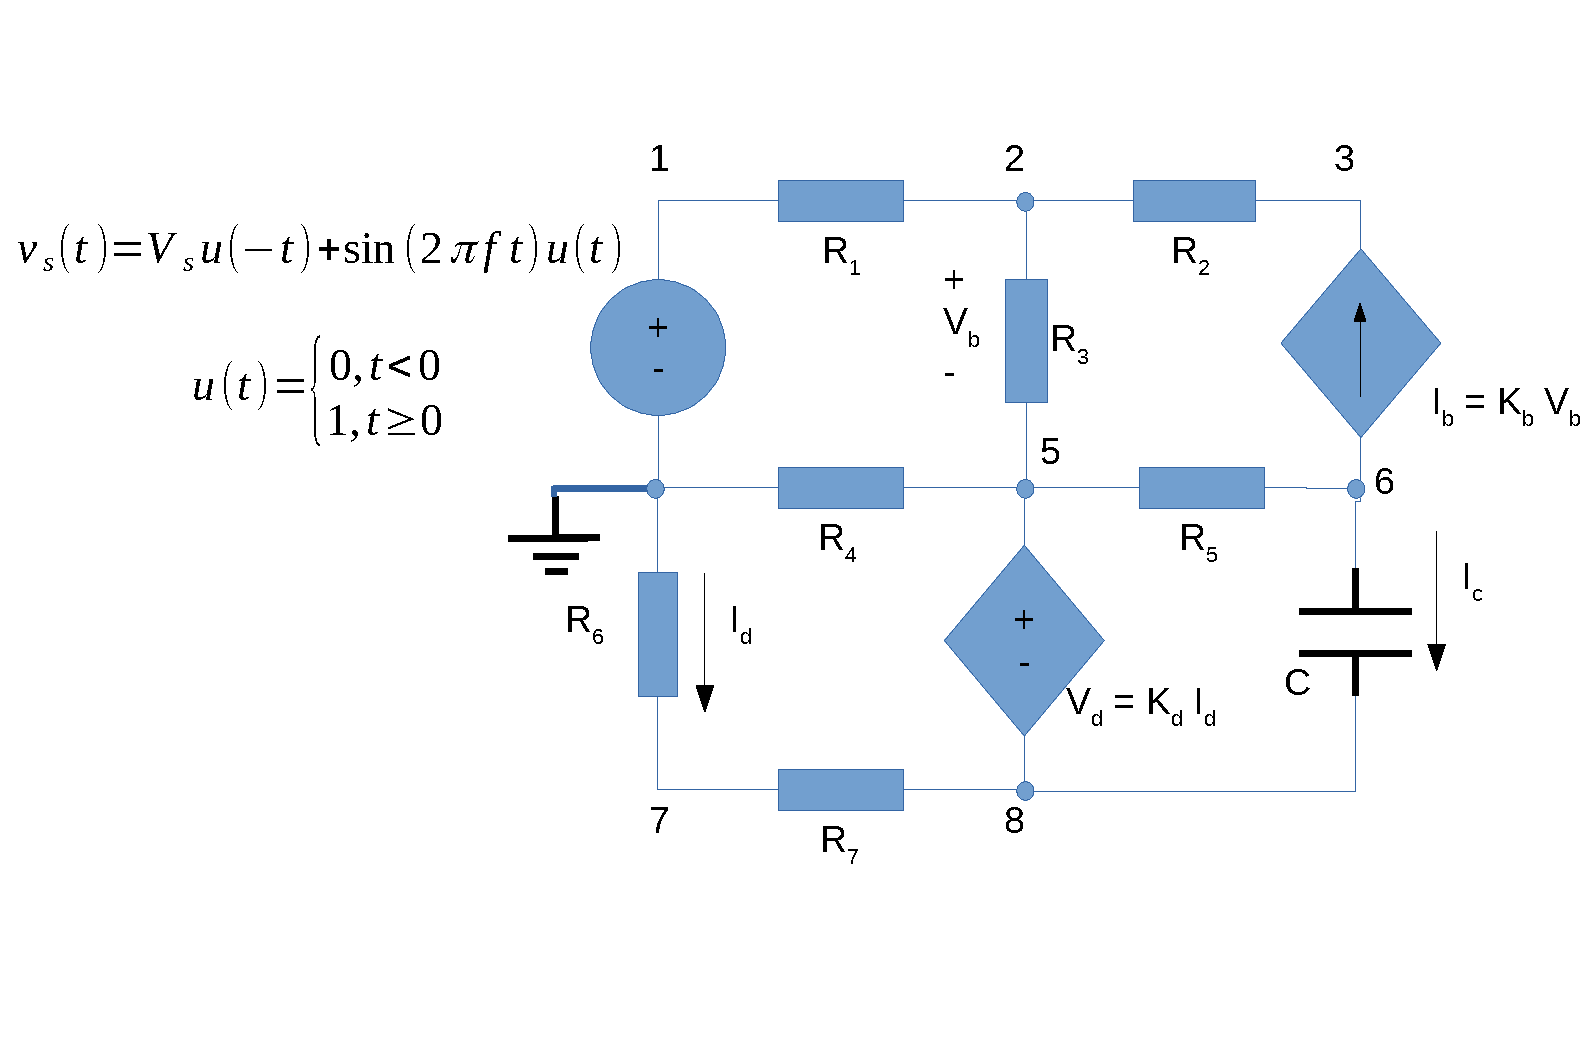
\includegraphics[width=0.8\linewidth]{rc.pdf}
\caption{The circuit under analysis}
\label{fig:rc}
\end{figure}

In Section \ref{sec:analysis1}, a theoretical analysis of the circuit is
presented, following a series of steps. In Section\ref{sec:simulation}, the circuit is analysed by
simulation, and the results are compared to the theoretical results obtained in
Section~\ref{sec:analysis}. The conclusions of this study are outlined in
Section~\ref{sec:conclusion}.






\section{Theoretical Analysis} \label{sec:analysis}

\subsection{Nodal Method at t$<$0}


In this Analysis, we enumerated the 8 nodes, from 1 to 8, as it's shown in Figure \ref{fig:rc}. We recognized that the GND is connected to node 4, so $V_{4}=0V$.Consequently $V_1$ is equal to the voltage on voltage source $v_s(t)$, and considering that we are working with the circuit at t<0, $v_s=V_1=V_s$.
In general, we considered node analysis on the nodes (using KCL and Ohm's Law, and considering that the currents are leaving the nodes) , to discover each voltage associated with each other. 
Since we are studying the circuit without a sinusoidal voltage source, for now, there's no variation over time of the voltage value on the capacitor, so there's no current flowing through it, $I_c=0A$, and the circuit behaves like an open circuit.
Another important aspect we considered while analyzing this circuit is that the potential difference between node 5 and node 8 is equal to $V_d$, so we can say that $V_d=V_5-V_8$. We can also apply KCL in the supernode made up by the linearly dependent voltage source ($V_d$), node 5 and node 8, and state that the sum of the currents leaving it is equal to 0 ($\frac{V_5}{R_4} + \frac{V_5-V_6}{R_5} + \frac{V_8-V_7}{R_7} + \frac{V_5-V_2}{R_3}=0$).

\begin{gather}
\begin{bmatrix}
1 & 0 & 0 & 0 & 0 & 0 & 0 & 0\\
-G_1 & G_1+G_2+G_3 & -G_2& 0 & -G_3 & 0 & 0 & 0\\
0 & -G_2-K_b & G_2 & 0 & K_b & 0 & 0 & 0\\
0 & 0 & 0 & 1 & 0 & 0 & 0 & 0\\
0 & 0 & 0 & 0 & 1 & 0 & K_d G_6 & -1\\
0 & -G_3 & 0 & 0 & G_3+G_4+G_5 & -G_5 & -G_7 & G_7\\
0 & K_b & 0 & 0 & -K_b-G_5 & G_5 & 0 & 0\\
0 & 0 & 0 & 0 & 0 & 0 & G_6+G_7 & -G_7
\end{bmatrix}
\begin{bmatrix}
 V_1\\
 V_2\\
 V_3\\
 V_4\\
 V_5\\
 V_6\\
 V_7\\
 V_8
\end{bmatrix}
=
\begin{bmatrix}
 V_S\\
 0\\
 0\\
 0\\
 0\\
 0\\
 0\\
 0
\end{bmatrix}
\end{gather}

Using the scientific programming language GNU Octave to solve the system above, we achieved the following:


\begin{table}[!htb]
    %\caption{Global caption}
    \begin{minipage}{.5\linewidth}
      
      \centering
        \begin{tabular}{|c|c|}
        \hline    
        {\bf Node} & {\bf V\textsubscript{i} [V]} \\ \hline
        \input{../mat/tabelaNodes1.tex}
        \end{tabular}
        \caption{Voltage values on each node (t$<$0)}
    \end{minipage}%
    \begin{minipage}{.5\linewidth}
      \centering
        
        \begin{tabular}{|c|c|}
        \hline    
        {\bf Branch} & {\bf I[A]} \\ \hline
        \input{../mat/tabelaIbranches1.tex}
        \end{tabular}
        \caption{Current values on each branch (t$<$0)}
    \end{minipage} 
\end{table}

\subsection{Circuit at t=0}
At t=0,  V\textsubscript{S}=0 and we considered the capacitor as a voltage source with a fixed potential difference $V\textsubscript{x} = V(6)-V(8)$, where V(6) and V(8) are the values obtained for t<0. Then, in order to obtain R\textsubscript{eq} , the equivalent resistance seen by the capacitor,  we ran nodal analysis once again, considering that there's a supernode that includes node 5, 6 and 8.
\begin{gather}
\begin{bmatrix}
1    & 0           & 0    & 0           & 0 & 0 & 0 & 0\\
-G_1 & G_1+G_2+G_3 & -G_2 & 0           & -G_3 & 0 & 0 & 0\\
0    & -G_2-K_b    & G_2  & 0           & K_b & 0 & 0 & 0\\
0    & 0           & 0    & 1           & 0 & 0 & 0 & 0\\
0    & 0           & 0    & 0           & 1 & 0 & K_d G_6 & -1\\
0    & 0           & 0    & 0           & 0 & 1 & 0 & -1\\
0    & 0           & 0    & 0           & 0 & 0 & G_6+G_7 & -G_7\\
0    & K_b-G_3     & 0    & G_3+G_4-K_b & 0 & 0 & -G_7 & G_7
\end{bmatrix}
\begin{bmatrix}
 V_1\\
 V_2\\
 V_3\\
 V_4\\
 V_5\\
 V_6\\
 V_7\\
 V_8
\end{bmatrix}
=
\begin{bmatrix}
 0\\
 0\\
 0\\
 0\\
 0\\
 V_x\\
 0\\
 0
\end{bmatrix}
\end{gather}


Then we used the following expression $I_x = \frac{V_6-V_5}{R_5} + K_b(V_2 - V_5)$, to obtain $I_x$ and we computed $R\textsubscript{eq} = V\textsubscript{x} / I\textsubscript{x}$. Lastly we obtained the value of the time constant $\tau=R_{eq}C$


The following tables show the voltages obtained on each node, as well as the data that caracterizes the capacitor.

\begin{table}[!htb]
    %\caption{Global caption}
    \begin{minipage}{.5\linewidth}
      
      \centering
        \begin{tabular}{|c|c|}
        \hline    
        {\bf Node} & {\bf V\textsubscript{i} [V]} \\ \hline
        \input{../mat/tabelaNodes2.tex}
        \end{tabular}
        \caption{Voltage values on each node (t=0)}
    \end{minipage}%
    \begin{minipage}{.5\linewidth}
      \centering
        
        \begin{tabular}{|c|c|}
        \hline    
        {\bf } & {\bf Value} \\ \hline
        \input{../mat/capacitor.tex}
        \end{tabular}
        \caption{Data that caracterizes the capacitor at t=0}
    \end{minipage} 
\end{table}
\newpage

\subsection{Transient Analysis for t$>$0}

When t$>$0, the voltages source has a sinusoidal behaviour, with frequency f=1kHz, which causes the voltage over the capacitor to have also an exponential decay (natural solution) superimposed with an sinusoidal behaviour with the same frequency as the source(forced solution).

\subsubsection{Natural Response}
It is know that the natural solution for a capacitor in a circuit takes the following form:
\begin{equation}
 V_n(t)=A e^{- \frac{t}{RC}}
\end{equation}

Imposing the boundary condition that at t=0, V\textsubscript{6}(0)= V\textsubscript x, we have:

\begin{equation}
 V_6(t)=V_x e^{- \frac{t}{R_{eq} C}}
\end{equation}

The following plot shows the natural solution within the first 20ms.
\begin{figure}[h] \centering
\includegraphics[width=0.5\linewidth]{t2-3.eps}
\caption{Natural solution t=[0,20]ms}
\label{fig:natural}
\end{figure}

\subsubsection{Total Response}

To compute the forced solution, we began by running nodal analysis once more in order to determine the phasor voltages in all nodes (achieving the complex amplitude and phase at each node). It is known that the phasor voltage in the first node is given by $V_S =1$ and the angular frequency is $w=2\pi f$, with $f=1000Hz$. Then we replaced C with its impedance $Z_c= \frac{V_c}{I_c}=\frac{1}{jwC}$, and we obtained that $I_c=jwC(V_6-V_8)$.

\begin{gather}
\begin{bmatrix}
1 & 0 & 0 & 0 & 0 & 0 & 0 & 0\\
-G_1 & G_1+G_2+G_3 & -G_2& 0 & -G_3 & 0 & 0 & 0\\
0 & -G_2-K_b & G_2 & 0 & K_b & 0 & 0 & 0\\
0 & 0 & 0 & 1 & 0 & 0 & 0 & 0\\
0 & 0 & 0 & 0 & 1 & 0 & K_d G_6 & -1\\
0 & K_b & 0 & 0 & -K_b-G_5 & G_5+jwC & 0 & -jwC\\
0 & 0 & 0 & 0 & 0 & 0 & G_6+G_7 & -G_7\\
0 & -G_3 & 0 & 0 & G_3+G_4+G_5 & -G_5-jwC & -G_7 & jwC+G_7\\
\end{bmatrix}
\begin{bmatrix}
 V_1\\
 V_2\\
 V_3\\
 V_4\\
 V_5\\
 V_6\\
 V_7\\
 V_8
\end{bmatrix}
=
\begin{bmatrix}
 1\\
 0\\
 0\\
 0\\
 0\\
 0\\
 0\\
 0
\end{bmatrix}
\end{gather}


Superimposing the natural solution with the forced solution we obtain the behavior of the capacitor over time.

\begin{figure}[h] \centering
\includegraphics[width=0.5\linewidth]{t2-5.eps}
\caption{Total solution t=[-5,20]ms (V(6) and V\textsubscript S )}
\label{fig:natural}
\end{figure}

As we can see, the capacitor is out of phase with the voltage source and there's a disruptance at t=0.

\begin{table}[!htb]
    %\caption{Global caption}
    \begin{minipage}{.5\linewidth}
      
      \centering
        \begin{tabular}{|c|c|}
        \hline    
        {\bf Node} & {\bf Amplitude} \\ \hline
        \input{../mat/amplitudes.tex}
        \end{tabular}
        \caption{Amplitude values on each node}
    \end{minipage}%
    \begin{minipage}{.5\linewidth}
      \centering
        
        \begin{tabular}{|c|c|}
        \hline    
        {\bf Node} & {\bf Phase} \\ \hline
        \input{../mat/phases.tex}
        \end{tabular}
        \caption{Current values on each node }
    \end{minipage} 
\end{table}



 
\newpage
\section{Simulation Analysis}
\label{sec:simulation}

The circuit under analysis was also simulated using Ngspice (revision 31) and maintaining the already mentioned node convention (figure \ref{fig:rc}). The forward subsections establish a comparison between theoretical and simulation results. The operating point analysis is already discussed in the theoretical anaylisis section and therefore it will not be mentioned again.

\subsection{Gain Stage}
From the simulation, one can conclude that a great deal of small-signal amplification occurs at the gain stage which is exactly this section's function. However, the signal has a huge DC deviation which is undesirable. Also, according to the rough estimates of the theoretical analysis, this stage has a huge output impedance which means that it enclosures the voltage out of the real output zone. This is why we need the output stage to impose enough signal amplitude arriving at the load. A graph of the signal at node C (the signal at the end of the gain stage) in a 100Hz regime is shown below. Bellow that is shown the frequency response of the gain stage's output which has some clear irregularities but a large bandwidth. These irregularities will also be corrected at the output stage. There is also the phase which is of lesser importance in a sound pitch context but is nonetheless displayed in figure \ref{fig:vpcoll}.

\begin{figure}[h] \centering
\includegraphics[width=0.4\linewidth]{vcoll.eps}%0.9
\vspace{-5mm}
\caption{Gain Stage output at 100Hz}
\label{fig:vcoll}
\end{figure}
\vspace{-5mm}

%\begin{figure}[h] \centering
%\includegraphics[width=0.9\linewidth]{vdbcoll.eps}
%\vspace{-5mm}
%\caption{Gain Stage output-frequency response}
%\label{fig:vdbcoll}
%\end{figure}

\begin{figure}[h] \centering
  \begin{minipage}{.45\textwidth}
    \includegraphics[width=.8\textwidth]{vdbcoll.eps}
    \caption{Gain Stage output-frequency response (amplitude)}
    \label{fig:vdbcoll}
  \end{minipage}%
    \hspace{2 mm}
  \begin{minipage}{.45\textwidth}
  \centering
    \includegraphics[width=.8\textwidth]{vpcoll.eps}
    \caption{Gain Stage output-frequency response (phase)}
    \label{fig:vpcoll}
      \end{minipage}%
\end{figure}

\newpage
\subsection{Output Stage}

The simulation shows that the output stage accomplishes its essential function. The output impedance is reduced (table \ref{tab:z}). And as shown in figure \ref{fig:vout} the output signal has a gain of roughly 50 (the input signal has an amplitude of 10 volts) and has no DC deviation and negligible distortion. The output signal also shows a large and plane bandwidth in the frequency response as desired (figure \ref{fig:vdbout}). The comparison between theoretical and simulation analysis will be discussed in detail in the conclusion section. It is also noted that the input impedance is high compared to the 100 Ohms of the input resistance which is also a desired feature.As already mentioned the phase dislayed in figure \ref{fig:vpout} is of minor importance.

%\begin{figure}[h] \centering
%\includegraphics[width=0.9\linewidth]{vout.eps}
%\vspace{-5mm}
%\caption{Output at 100Hz}
%\label{fig:vout}
%\end{figure}

\begin{figure}[h] \centering
  \begin{minipage}{.45\textwidth}
    \includegraphics[width=.8\textwidth]{vout.eps}
    \caption{Output frequency response - theoretical analysis}
    \label{fig:vout}
  \end{minipage}%
    \hspace{2 mm}
  \begin{minipage}{.45\textwidth}
  \centering
    \includegraphics[width=.8\textwidth]{vpout.eps}
    \caption{Output frequency response - theoretical analysis}
    \label{fig:vpout}
      \end{minipage}%
\end{figure}


\begin{figure}[h] \centering
  \begin{minipage}{.45\textwidth}
    \includegraphics[width=.8\textwidth]{vdbout.eps}
    \caption{Output frequency response - theoretical analysis}
    \label{fig:vdbout}
  \end{minipage}%
    \hspace{2 mm}
  \begin{minipage}{.45\textwidth}
  \centering
    \includegraphics[width=.9\textwidth]{frequencyresponse.eps}
    \caption{Output frequency response - theoretical analysis}
    \label{fig:compvdbout}
      \end{minipage}%
\end{figure}

\begin{table}[!htb]
  \begin{minipage}{.5\linewidth}
     \centering
  \begin{tabular}{|c|c|}
    \hline    
    {\bf Parameter} & {\bf Value} \\ \hline
    \input{../sim/zi_tab.tex}
    \input{../sim/zo_tab.tex}
 \end{tabular}
 \caption{Impedance (in Ohms) -  simulation analysis}
 \label{tab:z}
  \end{minipage}
    \hspace{2 mm}
    \begin{minipage}{.5\linewidth}
      \centering
        \begin{tabular}{|c|c|}
    \hline    
    {\bf Parameter} & {\bf Value} \\ \hline
     \input{../mat/total.tex}
 \end{tabular}
        \caption{Impedance (in Ohms) - theoretical analysis}
        \label{tab:compz}
    \end{minipage} 
\end{table}


\newpage
\subsection{Performance and Quality}
Besides the already presented input and output impedances, the performance and quality of this audio amplifier can be measured by cost, gain, lower-cutoff frequency, bandwidth, and merit (cost-benefit relation). In table \ref{tab:merit} these parameters are shown (and compared with the theoretical calculations). The gain is quite good (about 50 times) and the band of amplified frequencies contains all frequencies that a human can hear which is the maximum desirable band. At last, the merit is quite high. But the following should be stated: the figure of merit has some limitations. For example, if we reduced Rc by a factor of ten the figure of merit would become a great deal greater (more than its double), however, we would have an overall worse amplifier because it would have less gain. The merit would rise due to a great rise in the bandwidth but this expansion would to a region of frequencies that no human can hear, and who wants an amplifier with less gain just to have a uselessly large bandwidth?


\begin{table}[!htb]
  \begin{minipage}{.5\linewidth}
     \centering
  \begin{tabular}{|c|c|}
    \hline    
    {\bf Parameter} & {\bf Value} \\ \hline
    \input{../sim/merit_tab.tex}
 \end{tabular}
 \caption{Results of simulation analysis}
 \label{tab:merit}
  \end{minipage}%
    \hspace{2 mm}
    \begin{minipage}{.5\linewidth}
      \centering
        \begin{tabular}{|c|c|}
    \hline    
    {\bf Parameter} & {\bf Value} \\ \hline
    \input{../mat/merit.tex}
 \end{tabular}
        \caption{Results of theoretical analysis}
        \label{compmerit}
    \end{minipage} 
\end{table}


%\newpage
\section{Conclusion}
\label{sec:conclusion}
In this laboratory assignment, the objective of build and analyse the working principle of an audio amplifier was successfully achieved.
The cost of the circuit was xxx MU and the merit xxx.
Comparing the results from both the theoretical analysis using Octave and the circuit simulation using ngspice, we can see in the following figure and table, that they appear to slightly differ.

In both analysis the output voltage was close to $12 V$ and had a small ripple. The shape of the graphs obtained in both of them was very similar and the frequencies and the phases appear to be the same.

However, the theoretical model gives a lower value for both the input and output impendance and a smaller bandwidth, but a lot bigger value for the gain. 

We can conclude that there are some differences between the theoretical and simulation analysis. These variations are due to the various aproximations made in the theoretical analysis, in the ideal transistor model for example, while the simulation assume that the circuit is linear and uses a comparatively accurate spice model.  


%merry chrislter
%$https://www.youtube.com/watch?v=_Z-Nu351j58$

%\lipsum[1-1]

%\cleardoublepage

% ----------------------------------------------------------------------
%  Bibliography
% ----------------------------------------------------------------------
%\addcontentsline{toc}{section}{\bibname}
%\bibliographystyle{abbrvunsrtnat} % <<<<< SELECT IF USING REFERENCES BY NUMBER (CITATION ORDER)
%\bibliography{../../../BIBfile.bib}

% ----------------------------------------------------------------------
\end{document}
% ----------------------------------------------------------------------
